\chapter{One-dimensional symmetric phases protected by frieze symmetries}

\section{Synopsis}
In \cref{sec:1Dphases} we reviewed the classification of SPT phases protected by \emph{internal} symmetries acting in an on-site manner. The present project extends this classification to include quasi-one-dimensional spatial symmetries. These are encoded in the so-called frieze groups, of which there are seven. Crucially, by following an approach closely analogous to that of \cref{sec:1Dphases} and studying the action of the symmetry on an injective MPS, we find that these SPT phases are classified by the second cohomology group of the protecting symmetry group over $\rU(1)$, with the additional feature that \emph{orientation-reversing} group elements --- encoding spatial reflection, for instance --- act on $\rU(1)$ via complex conjugation. Additionally, we provide MPS normal forms for each of these phases and explicit MPS representations directly in terms of representative cocycles. Also, we discuss an algorithm that computes cohomology groups of any order and corresponding representative cocycles, including in the presence of non-trivial group action.

\section{Reference}

% TODO make compatible with reference style
%\cite{Vancraeynest2022}
\textit{One-dimensional symmetric phases protected by frieze symmetries}, \par\noindent
\textbf{B. Vancraeynest-De Cuiper}, J. C Bridgeman, N. Dewolf, J. Haegeman, F. Verstraete \par\noindent
\href{https://doi.org/10.1103/PhysRevB.107.115123}{Physical Review B \textbf{107} (11), 115123 (2023)}, \href{https://doi.org/10.48550/arXiv.2202.12880}{arXiv:2202.12880}
\section{Contributions of the author}
The project underlying this paper grew out of the Master's thesis of N. Dewolf. Therein the classification of SPT phases protected by frieze symmetries was initiated and the framework established. The present author completed this classification and their representative cocycles, in full generality, and co-wrote most of the manuscript.
\section{One-dimensional symmetric phases protected by frieze symmetries}

% TODO: fix page numbering
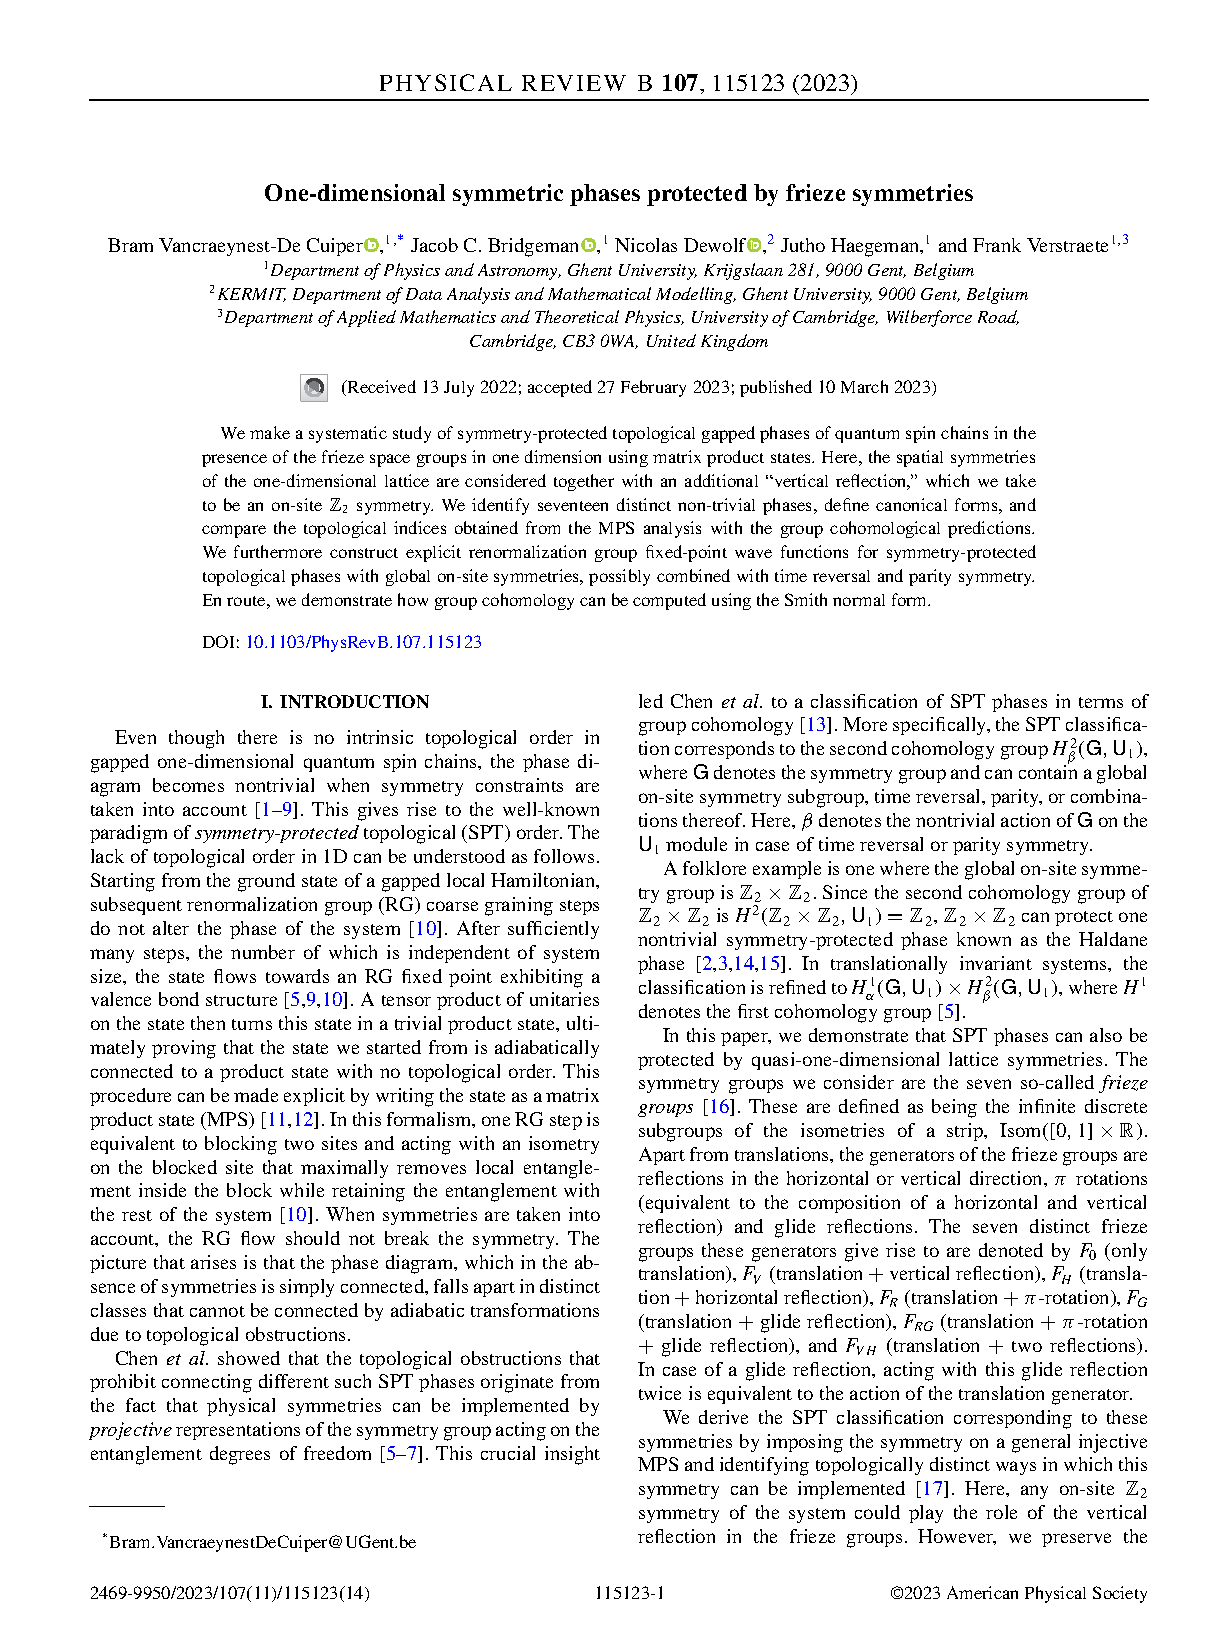
\includepdf[pages=-, trim=20 40 15 15, clip=true, frame=false, noautoscale=true, width=1.14\headwidth, offset=-1mm 5mm]{papers/frieze}